\section{Avantages du traitement des données}
\paragraph{}
Le traitement des données est important pour de multiples raisons.
Premièrement, il est important d'éliminer le bruit ou tout type d'information non essentielle des données.
Deuxièmement, nous pouvons examiner comment nous pouvons tirer davantage d'informations de nos ``données brutes''.
% Data processing is important because of multiple reasons.
% First, it is important to remove noise or any kind of unessential information from or data.
% Secondly, we can look into how we can derive more information from our ``raw data''

\section{Travailler uniquement avec les yeux}
\label{data-processing:eyes}
\paragraph{}
Dans certaines des expériences suivantes, je me suis concentré sur l'extraction des yeux d'une image.
Pour cela, j'ai utilisé deux bibliothèques: \lstinline{dlib} et \lstinline{imutils}.
Sur la base des repères faciaux présentés dans l'introduction \ref{figure:facial-landmarks}, j'ai extrait uniquement la partie de l'image décrite par les repères faciaux pour les yeux.
% In some of the following experiments, I focused on only extracting the eyes from an image.
% For this, I used two libraries: dlib and imutils.
% Based on the facial landmarks that were presented in the introduction \ref{figure:facial-landmarks}, I extracted only the image portion described by the facial landmarks for the eyes.

\begin{lstlisting}[language=Python, caption=Extraire les yeux]
def extract_eyes(cv2_image):
    """Returns a list of images that contain the eyes extracted from the original image.

    First result is the left eye, second result is the right eye."""
    global stuff_was_initialized, face_detector, face_predictor
    if stuff_was_initialized == False:
        initialize_stuff()

    gray_image = Utils.convert_to_gray_image(cv2_image)
    rects = face_detector(gray_image, 0)
    if len(rects) > 0:
        shape = face_predictor(gray_image, rects[0])
        shape = face_utils.shape_to_np(shape)

        eyes = []
        for eye in ["left_eye", "right_eye"]:
            # get the points for the contour
            (eye_start, eye_end) = face_utils.FACIAL_LANDMARKS_IDXS[eye]
            contour = shape[eye_start:eye_end]
            # get the upper left point, lower right point for this eye
            start = [min(contour, key=lambda x: x[0])[0],
                    min(contour, key=lambda x: x[1])[1]]
            end = [max(contour, key=lambda x: x[0])[0],
                max(contour, key=lambda x: x[1])[1]]
            # extract the current eye
            eyes.append(cv2_image[start[1]:end[1], start[0]:end[0]])
        return eyes

    return None
\end{lstlisting}

\clearpage
\paragraph{}
Comme nous ne nous intéressons qu'au contraste entre l'iris et la pupille, j'ai ensuite appliqué un \emph{seuil binaire} sur l'image grise de l'œil pour souligner la façon dont la pupille est située par rapport à l'ensemble de l'œil.
% Since we are only interested in the contrast between the iris and the pupil, I afterwards applied a \emph{binary threshold} on the eye's gray image to emphasize on how the pupil is situatied relative to the whole eye.

\begin{lstlisting}[language=Python, caption=Application d'un seuil binaire]
def get_binary_thresholded_image(cv2_image):
    img = convert_to_gray_image(cv2_image)
    img = cv2.medianBlur(img, 5)
    img = cv2.adaptiveThreshold(
        img, 255, cv2.ADAPTIVE_THRESH_GAUSSIAN_C, cv2.THRESH_BINARY, 11, 2)
    return img
\end{lstlisting}

\begin{figure}[H]
    \centering
    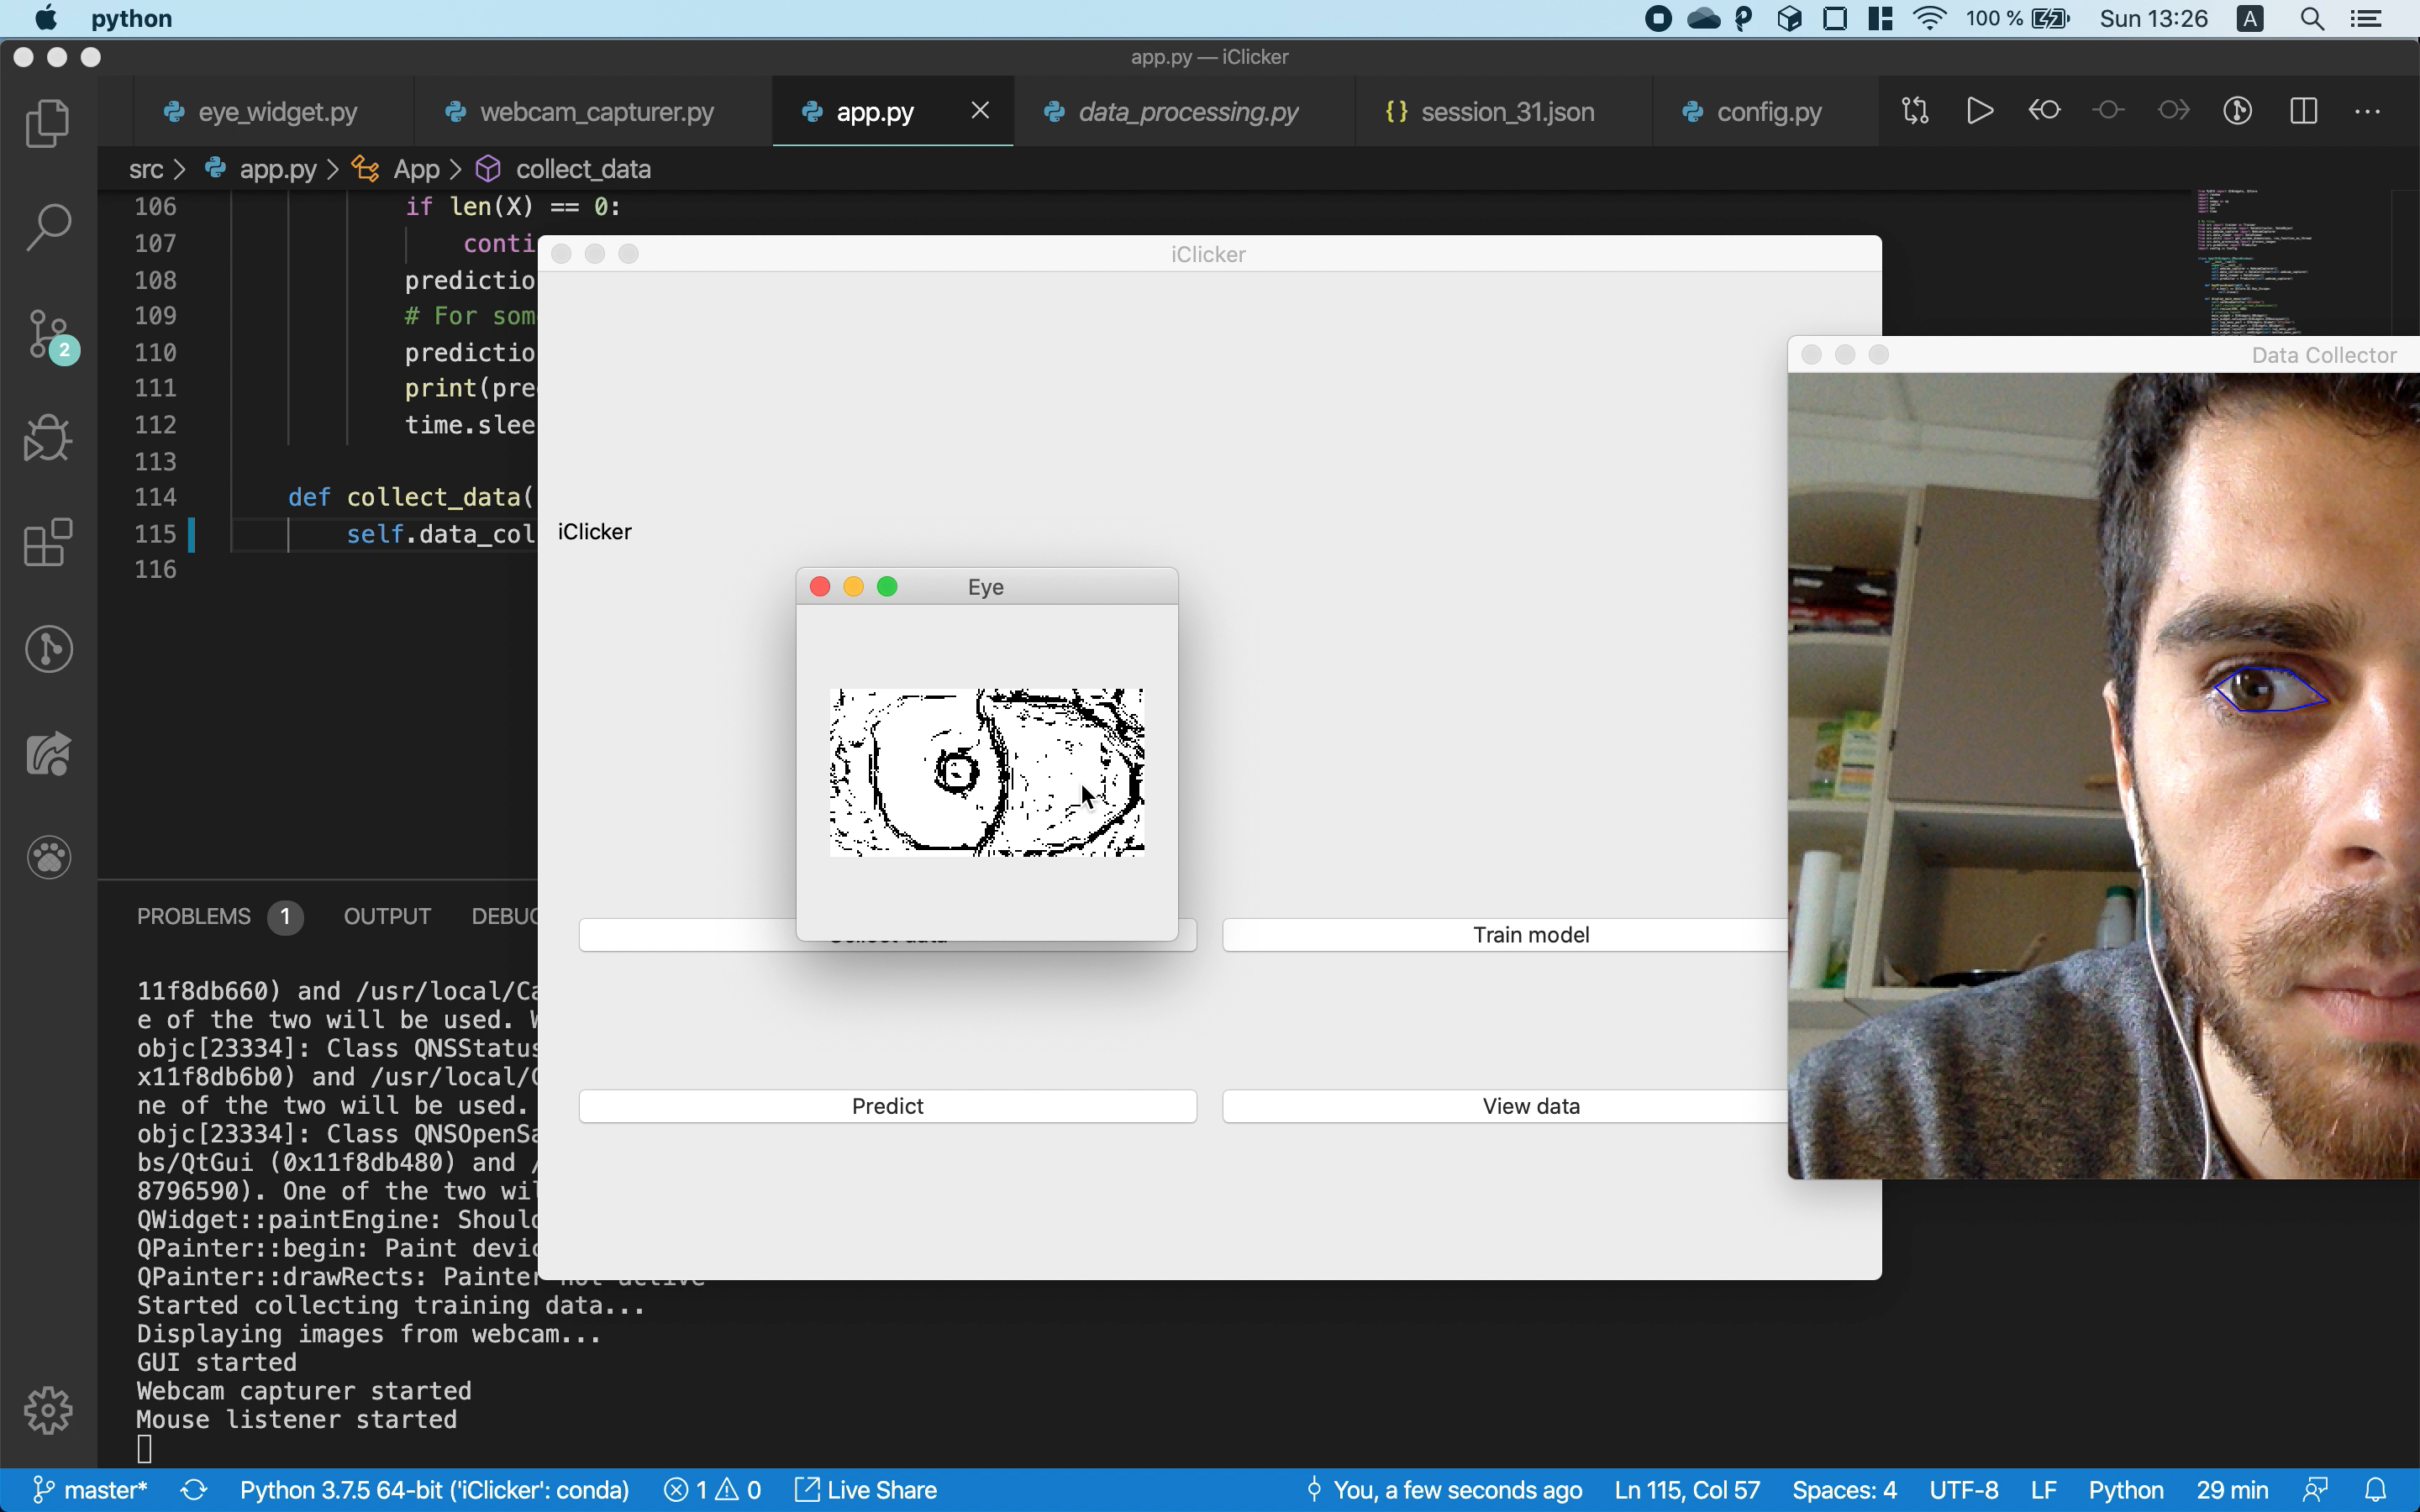
\includegraphics[width=\textwidth/2 - 5pt]{eye_binary_threshold.png}
    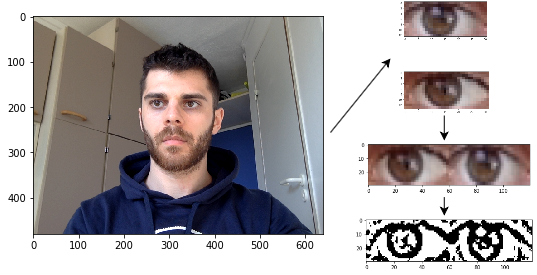
\includegraphics[width=\textwidth/2 - 5pt]{threshold_process.png}
    \caption{Obtenir des données sur les yeux}
\end{figure}

\section{En utilisant seulement le visage}
\paragraph{}
% My next idea was to use the face and give this as input to a CNN.
% This is how the data processing looks like:
Mon idée suivante était d'utiliser le visage et de le donner en entrée à une CNN.
Voici à quoi ressemble le traitement des données :
\begin{figure}[H]
    \centering
    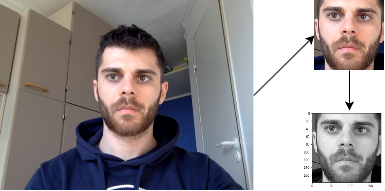
\includegraphics{extract_face_process.png}
    \caption{Extraire le visage}
    \label{fig_extracted_faces}
\end{figure}

\paragraph{}
% The final image is a square containing the face extracted from the images, converted to grayscale.
% It was also normalised to take values between $0$ and $1$.
% Afterwards, depending on the grid size, the images were labeled with the cell number corresponding to where the user was looking.

L'image finale est un carré contenant le visage extrait des images, converti en niveaux de gris.
Elle a également été normalisée pour prendre des valeurs entre $0$ et $1$.
Ensuite, en fonction de la taille de la grille \ref{grid-example}, les images ont été étiquetées avec le numéro de la cellule correspondant à l'endroit où l'utilisateur regardait.

\begin{lstlisting}[language=Python, caption = Extraction du visage en Python3]
def extract_face(cv2_image):
"""Returns the face part extracted from the image"""
global stuff_was_initialized, face_detector
if stuff_was_initialized == False:
    initialize_stuff()

gray_image = Utils.convert_to_gray_image(cv2_image)
rects = face_detector(gray_image, 0)
if len(rects) > 0:
    # only for the first face found
    (x, y, w, h) = face_utils.rect_to_bb(rects[0])
    return cv2_image[y:y+h, x:x+w]
return None
\end{lstlisting}
% Un travail en cours porte sur la façon dont je peux utiliser le visage entier comme intrant pour un Réseau Neuronal Convolutif et sur la question de savoir si je dois y appliquer un traitement quelconque.
% Je reviendrai lorsque j'aurai des résultats à ce sujet, car il s'agit d'un travail en cours.
% A current work in progress is researching on how I can use the whole face as an input for a Convolutional Neural Network and whether I should apply any kind of processing to it or not.
% I will come back when I have some results for this, as this is work in progress.

\section{``Bandeau oculaire''}
\paragraph{}
Next, I'll try to use only the eyes as data, but without modifying them.
Here's how that looks:

\begin{figure}[H]
    \centering
    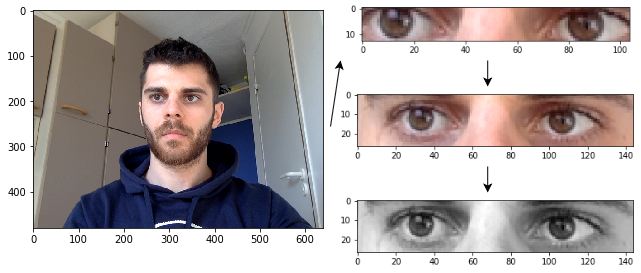
\includegraphics[width = \textwidth]{extract_eye_strip_process.png}
    \caption{Extraction de ``bandeau oculaire''}
    \label{fig_extracting_eye_strip}
\end{figure}

\paragraph{}
I extract both eyes from the detected face, I expand the bounding box to have more information, then I convert it to grayscale and normalise it.

\begin{lstlisting}[language=Python, caption=Extraction de ``bandeau oculaire'' en Python3]
def extract_eye_strip(cv2_image):
    """Returns a horizontal image with the two eyes extracted from the image"""
    global stuff_was_initialized, face_detector, face_predictor
    if stuff_was_initialized == False:
        initialize_stuff()

    gray_image = Utils.convert_to_gray_image(cv2_image)
    rects = face_detector(gray_image, 0)
    if len(rects) > 0:
        # only for the first face found
        shape = face_predictor(gray_image, rects[0])
        shape = face_utils.shape_to_np(shape)
        (left_eye_start,
         left_eye_end) = face_utils.FACIAL_LANDMARKS_IDXS["left_eye"]
        (right_eye_start,
            right_eye_end) = face_utils.FACIAL_LANDMARKS_IDXS["right_eye"]
        # get the contour
        start, end = min(left_eye_start, right_eye_start), max(
            left_eye_end, right_eye_end)
        strip = shape[start:end]
        # get the upper left point, lower right point
        start = [min(strip, key=lambda x: x[0])[0],
                 min(strip, key=lambda x: x[1])[1]]
        end = [max(strip, key=lambda x: x[0])[0],
               max(strip, key=lambda x: x[1])[1]]
        # go a little outside the bounding box, to capture more details
        distance = (end[0] - start[0], end[1] - start[1])
        # 20 percent more details on the X axis, 60% more details on the Y axis
        percents = [20, 60]
        for i in range(0, 2):
            start[i] -= int(percents[i]/100 * distance[i])
            end[i] += int(percents[i]/100 * distance[i])
        return cv2_image[start[1]:end[1], start[0]:end[0]]
    return None
\end{lstlisting}